\chapter{RLC Circuits, Resonance, and the Quality Factor}
\label{ch:rlc-resonance}

Combining an inductor and a capacitor in the same circuit produces one of
the single most important phenomena in all of radio: \textbf{resonance}.
Every tuned circuit, every antenna, every IF filter, and every
transmitter's output network relies on the ideas in this chapter.

\section{Why L and C Together Are Special}

Recall from Chapters~\ref{ch:capacitors}--\ref{ch:inductors} that
$X_C = 1/(\omega C)$ falls with frequency while $X_L = \omega L$ rises
with frequency, and that they have opposite sign in complex impedance
notation ($Z_C = -jX_C$, $Z_L = +jX_L$). This means there is always some
frequency at which $X_L$ and $X_C$ are exactly equal in magnitude ---
and, because of their opposite signs, they \emph{cancel} at that
frequency. This special frequency is the circuit's \textbf{resonant
frequency}, $f_0$.

\section{Series Resonance}

For a series RLC circuit, total impedance is
\[
Z = R + j(X_L - X_C) = R + j\left(\omega L - \frac{1}{\omega C}\right).
\]
At resonance, $X_L = X_C$, so the reactive part vanishes and
$Z = R$ --- the impedance is purely resistive and at its \textbf{minimum}
possible value. This means current through a series RLC circuit is at
its \emph{maximum} at resonance, for a given applied voltage. Setting
$X_L = X_C$ and solving for frequency gives the single most-used formula
in RF circuit design:
\[
\boxed{f_0 = \frac{1}{2\pi\sqrt{LC}}}
\]

\begin{examplebox}[Resonant frequency]
Find the resonant frequency of a 10\,$\mu$H inductor and a 100\,pF
capacitor in series.

\emph{Solution.}
\[
f_0 = \frac{1}{2\pi\sqrt{LC}} = \frac{1}{2\pi\sqrt{10\times10^{-6}\times100\times10^{-12}}} \approx 5.03\,\text{MHz}.
\]
\end{examplebox}

Away from resonance, the series circuit's impedance rises (dominated by
whichever reactance is larger), so current falls off on either side of
$f_0$ --- a series RLC circuit is inherently a \textbf{band-pass}
response when current (or voltage across $R$) is the output of interest.

\section{Parallel Resonance (the ``Tank Circuit'')}

An inductor and capacitor in parallel (an \textbf{LC tank circuit}) show
the complementary behavior. At resonance, the two branch currents
($I_L$ through the inductor, $I_C$ through the capacitor) are equal in
magnitude and $180\degree$ out of phase, so they cancel in the external
circuit --- ideally, at resonance, a parallel LC combination draws
\emph{zero} net current from the source and presents an
\emph{infinite} impedance (limited in practice only by real-world
losses, discussed below). This makes a parallel LC tank behave as a
band-\emph{reject} (notch) element as seen from outside, or,
equivalently, as a very high-impedance load exactly at $f_0$ --- the
mechanism used to select one frequency in an oscillator or amplifier
tank circuit while presenting low impedance to all other frequencies.
The resonant frequency formula is identical: $f_0 = 1/(2\pi\sqrt{LC})$.

\begin{keyidea}[Energy exchange at resonance]
At resonance, energy sloshes back and forth between the capacitor's
electric field and the inductor's magnetic field every half-cycle,
rather than being repeatedly drawn from (and returned to) the source.
This is why a well-designed (low-loss) tank circuit, once excited, can
``ring'' at its resonant frequency for many cycles even with the drive
removed --- the same physical principle as a bell continuing to ring
after being struck.
\end{keyidea}

\section{The Quality Factor, Q}
\label{sec:q-factor}

Real inductors and capacitors have loss (mostly resistive: wire
resistance, core loss, dielectric loss). The \textbf{quality factor}
$Q$ measures how ``lossless'' a resonant circuit is --- the ratio of
energy stored to energy dissipated per cycle:
\[
Q = 2\pi\,\frac{\text{energy stored}}{\text{energy dissipated per cycle}}.
\]
For a series RLC circuit,
\[
\boxed{Q = \frac{X_L}{R} = \frac{X_C}{R} = \frac{1}{R}\sqrt{\frac{L}{C}} = \frac{2\pi f_0 L}{R}}
\]
(evaluated at resonance, where $X_L=X_C$). For a parallel RLC circuit
(loss modeled as a resistance in parallel with the tank),
\[
Q = \frac{R}{X_L} = R\sqrt{\frac{C}{L}}.
\]

\begin{keyidea}[What Q buys you]
A \textbf{high-Q} circuit has a narrow, sharply peaked resonance ---
excellent selectivity (able to separate closely spaced signals) but also
unforgiving of small component drift and lossier to build. A
\textbf{low-Q} circuit has a broad, gentle resonance --- easier to build
and more tolerant of component tolerance, but poorer at rejecting
nearby unwanted signals. Receiver IF filters favor high Q; broadband
matching networks often favor deliberately lower Q.
\end{keyidea}

\section{Bandwidth and the Resonance Curve}

$Q$ directly sets the \textbf{bandwidth} $B$ of the resonance --- the
range of frequencies over which the response stays within
$3\,\text{dB}$ (half-power) of its peak value:
\[
\boxed{B = \frac{f_0}{Q}}
\]

\begin{center}
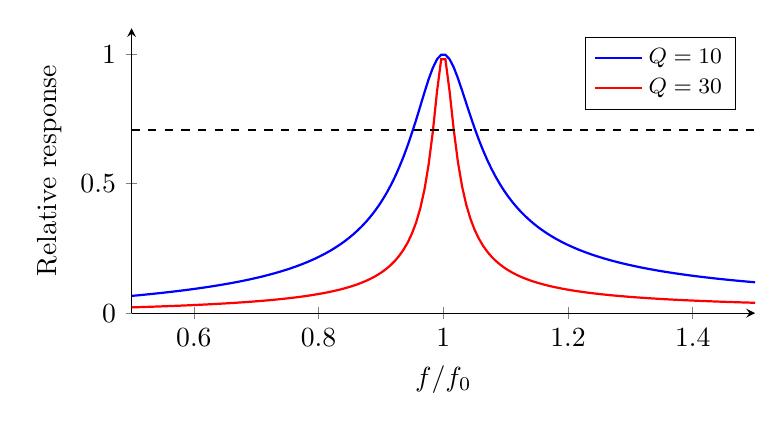
\begin{tikzpicture}
\begin{axis}[width=9.5cm,height=5.2cm,xlabel={$f/f_0$},ylabel={Relative response},
  xmin=0.5,xmax=1.5,ymin=0,ymax=1.1,domain=0.5:1.5,samples=150,
  axis lines=left,legend pos=north east, legend style={font=\footnotesize}]
\addplot[thick,blue] {1/sqrt(1+(10*(x-1/x))^2)};
\addlegendentry{$Q=10$}
\addplot[thick,red] {1/sqrt(1+(30*(x-1/x))^2)};
\addlegendentry{$Q=30$}
\draw[dashed] (axis cs:0.5,0.707) -- (axis cs:1.5,0.707) node[right,font=\footnotesize] {$-3$dB};
\end{axis}
\end{tikzpicture}
\end{center}

\begin{examplebox}[Bandwidth from Q]
A series-tuned circuit resonates at 7.1\,MHz with $L=2.5\,\mu$H,
$C=200\,\text{pF}$, and series resistance $R=3\,\Omega$. Find $Q$ and the
bandwidth.

\emph{Solution.}
\[
X_L = 2\pi f_0 L = 2\pi\times7.1\times10^6\times2.5\times10^{-6} \approx 111.5\,\Omega,
\]
\[
Q = \frac{X_L}{R} = \frac{111.5}{3} \approx 37.2, \qquad
B = \frac{f_0}{Q} = \frac{7.1\,\text{MHz}}{37.2} \approx 191\,\text{kHz}.
\]
\end{examplebox}

\section{Applications of Resonance in Radio}

\begin{itemize}
\item \textbf{Receiver front-end and IF selectivity}: tuned circuits
select the wanted signal and reject adjacent ones (Chapter~\ref{ch:receivers}).
\item \textbf{Transmitter output (tank) circuits}: convert an amplifying
device's output into a clean sinusoidal RF signal while suppressing
harmonics.
\item \textbf{Antenna tuning units}: use variable L and C to present a
resonant, well-matched impedance to a transmitter (Chapter~\ref{ch:transmission-lines}).
\item \textbf{Oscillators}: an LC tank sets the operating frequency of
many RF oscillator designs.
\item \textbf{Filters}: cascading multiple resonant sections builds the
band-pass, low-pass, and high-pass filters used throughout receivers and
transmitters (Chapter~\ref{ch:error-control} and Chapter~\ref{ch:receivers}).
\end{itemize}

\begin{quickreview}
\item Resonance occurs where $X_L = X_C$; $f_0 = 1/(2\pi\sqrt{LC})$ for
both series and parallel RLC circuits.
\item Series resonance: minimum impedance, maximum current (band-pass
behavior for current/output-across-R).
\item Parallel resonance (tank): maximum impedance, minimum line current
(band-reject as seen from outside; selects one frequency in a tank
application).
\item $Q = X/R$ at resonance; higher $Q$ means narrower bandwidth,
$B = f_0/Q$, and better selectivity but less tolerance and more loss
sensitivity.
\end{quickreview}

\begin{practiceproblems}
\item Find the resonant frequency of $L=4\,\mu$H, $C=68\,$pF.
\item A parallel tank has $R=10\,\text{k}\Omega$ (representing loss),
$L=1\,\mu$H, $C=400\,$pF. Find $f_0$ and $Q$.
\item A series-tuned circuit has $Q=50$ at $f_0=14.1\,$MHz. Find its
bandwidth.
\item Explain why a high-$Q$ circuit is more sensitive to small
component value changes than a low-$Q$ circuit.
\item A receiver needs to separate two signals 5\,kHz apart at
7.05\,MHz. Estimate the minimum $Q$ needed for a single resonant circuit
to provide meaningful separation (bandwidth on the order of the spacing).
\end{practiceproblems}
